Uma amostra de \chemfig{C_2H_4}(g) foi colocada em um recipiente rígido de 2,0 L previamente evacuado e aquecido de 300 K a 450 K.
A pressão da amostra é medida e representada no gráfico abaixo:

\begin{center}
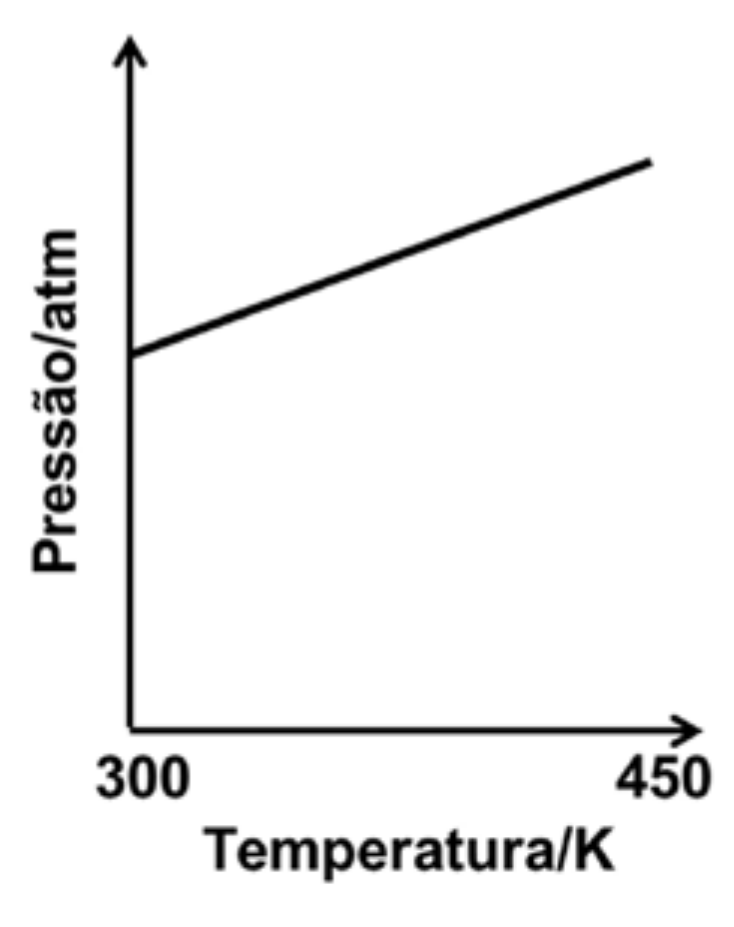
\includegraphics[width=0.2\textwidth]{figure1.png}
\end{center}

\begin{enumerate}[label = (\alph*)]
	\item  Descreva duas razões pelas quais as alterações de pressão e temperatura do \chemfig{C_2H_5Cl}(g) aumentam.
		Suas descrições devem estar em termos do que ocorre em nível molecular.
	\item \chemfig{C_2H_4}(g) reage prontamente com \chemfig{HCl}(g) para produzir \chemfig{C_2H_5Cl}(g), conforme representado pela seguinte equação. 

	\begin{center}
	\schemestart
	\chemfig{C_2H_4}(g) + \chemfig{HCl} \arrow{->} \chemfig{C_2H_5Cl}(g) \qquad $\Delta H^\circ = -72,6$ kJ$\cdot$mol$^{-1}$
	\schemestop
	\end{center}

	\item Propõe-se que a formação de \chemfig{C2H5Cl}(g) se dar via mecanismo de reação em duas etapas seguintes. 
	
	Etapa 1:
	\schemestart
	\chemfig{C_2H_4}(g) + \chemfig{HCl}(g) \arrow{->} \chemfig{C_2H_5^+}(g) + \chemfig{Cl^{-}}(g)
	\schemestop
	
	Etapa 2:
	\schemestart
	\chemfig{C_2H_5^+}(g) + \chemfig{Cl^{-}}(g) \arrow{->} \chemfig{C_2H_5Cl}
	\schemestop

	\item Identifique um dos intermediários no mecanismo de reação acima. 
	\item Esboce o gráfico da curva que mostra as mudanças de energia que ocorrem durante o progresso da reação.
		A curva deve ilustrar o mecanismo em duas etapas proposta e o comportamento  da variação de entalpia da reação.
		Indique claramente o que significa cada eixo, a energia de ativação ($E_a$) para a etapa determinante da velocidade na reação e os reagentes e produtos na equação global.

\end{enumerate}
